\sectionframe{Recap}
\section{Recap}

\begin{frame}{Complex Model}
    \begin{itemize}
        \item We started with a complex model describing the dynamics of a power converter
        \item It exhibited interesting dynamics we want to understand
    \end{itemize}
    \begin{figure}
        \includegraphics[width=0.3 \textwidth]{99_Yunus/2D_Period_Zoomed/result.png}
    \end{figure}

    \todo{mention type B parameter regions}
\end{frame}

\begin{frame}{Original Model (1/3)}
    \vspace{-2.0em}
    \begin{align}
        \theta      & \mapsto  F(\theta) \mod 2 \pi
        \\
        F(\theta)   & = \begin{cases}
                            F_1(\theta) & \text{if } q \cdot \cos(\theta) > 0 \\
                            F_2(\theta) & \text{if } q \cdot \cos(\theta) < 0
                        \end{cases}
        \\
        F_1(\theta) & = \begin{cases}
                            \theta + z_{L_+} + z_1 & \text{if } z_{L_+} < z_{L_0} \\
                            \theta + z_{L_0} + z_2 & \text{if } z_{L_+} > z_{L_0}
                        \end{cases}
        \\
        F_2(\theta) & = \begin{cases}
                            \theta + z_{R_+} + z_3 & \text{if } z_{R_+} < z_{R_0} \\
                            \theta + z_{R_0} + z_4 & \text{if } z_{R_+} > z_{R_0}
                        \end{cases}
    \end{align}

    \pause
    \vspace{2em}
    This looks ok, but how are these values defined?
    \begin{align*}
        z_1, z_2, z_3, z_4, z_{L_+}, z_{L_-}, z_{R_+}, \text{ and } z_{R_0}
    \end{align*}
\end{frame}

\begin{frame}{Original Model (2/3)}
    The smallest non-negative solutions to the following implicit equations
    \begin{subequations}
        \begin{align}
            (q \cdot \cos(\theta) + \mu \cdot \chi) \cdot e^{\lambda \cdot z_{L_+}}
             & = q \cdot \cos(\theta + z_{L_+} + z_1) + \mu \cdot \chi \\
            (q \cdot \cos(\theta) + \mu \cdot \chi) \cdot e^{\lambda \cdot z_{L_0}}
             & = q \cdot \cos(\theta + z_{L_0} + z_1) - \mu \cdot \chi \\
            (q \cdot \cos(\theta) + \mu \cdot \chi) \cdot e^{\lambda \cdot z_{R_+}}
             & = q \cdot \cos(\theta + z_{R_+} + z_1) + \mu \cdot \chi \\
            (q \cdot \cos(\theta) + \mu \cdot \chi) \cdot e^{\lambda \cdot z_{R_0}}
             & = q \cdot \cos(\theta + z_{R_0} + z_1) - \mu \cdot \chi
        \end{align}
    \end{subequations}
    \vspace{-2em}
    \begin{subequations}
        \begin{align}
            (q \cdot \cos(\theta + z_{L_+}) + \chi + 1) \cdot e^{\lambda \cdot z_1} - 1
             & = q \cdot  \cos(\theta + z_{L_+} + z_1) + \mu \cdot \chi \\
            (q \cdot \cos(\theta + z_{L_0}) + \chi + 1) \cdot e^{\lambda \cdot z_2} + 1
             & = q \cdot  \cos(\theta + z_{L_0} + z_2) - \mu \cdot \chi \\
            (q \cdot \cos(\theta + z_{R_+}) + \chi + 1) \cdot e^{\lambda \cdot z_3} - 1
             & = q \cdot  \cos(\theta + z_{L_+} + z_3) + \mu \cdot \chi \\
            (q \cdot \cos(\theta + z_{R_0}) + \chi + 1) \cdot e^{\lambda \cdot z_4} + 1
             & = q \cdot  \cos(\theta + z_{R_0} + z_4) - \mu \cdot \chi
        \end{align}
    \end{subequations}
\end{frame}

\begin{frame}{Original Model (3/3)}
    \vspace{-3.0em}
    \begin{align}
        \chi    & = \dfrac{R \cdot \chi_0}{\beta \cdot E_0} \\
        \lambda & = \dfrac{-R}{L \cdot 2 \cdot \pi \cdot f} \\
        q       & = \dfrac{R \cdot V_m}{\beta \cdot E_0}
    \end{align}

    Normalized and varied Parameters:
    \begin{align*}
        E_0, \chi_0
    \end{align*}

    Symmetry in this model:
    \begin{align}
        F(\theta + \pi) = F(\theta) + \pi \mod 2 \pi
    \end{align}

    \begin{flushright}
        Definition and symmetry from \cite{akyuz2022}
    \end{flushright}
\end{frame}

\begin{frame}{Minimal Reproducing Model Dynamics}
    \begin{figure}
        \includegraphics[width=0.3 \textwidth]{99_Yunus/2D_Period_Zoomed/result.png}
        \qquad
        \includegraphics[width=0.3 \textwidth]{60_MinimalRepr/2D_Period_Whole_noPoints/result.png}
    \end{figure}
    With this simpler model, we explained the structures
\end{frame}

\begin{frame}{Definition of the Minimal Reproducing Model (1/2)}
    \vspace{-3.0em}
    \begin{align}
        x \mapsto f(x) \mod 1
    \end{align}

    \begin{align}
        f(x) & = \begin{cases}
                     g(x)                                        & \text{ if } x < \frac{1}{2} \\
                     g\left(x - \frac{1}{2}\right) + \frac{1}{2} & \text{ else}
                 \end{cases}
    \end{align}

    \begin{align}
        g(x) & = \begin{cases}
                     l(x) = a_L \cdot x^2 + b_L \cdot x + c_L & \text{ if } x < \frac{1}{4} \\
                     r(x) = b_R \cdot x + c_R                 & \text{ else}
                 \end{cases}
    \end{align}
\end{frame}

\begin{frame}{Definition of the Minimal Reproducing Model (2/2)}
    \vspace{-1em}
    \begin{columns}
        \begin{column}{.7 \textwidth}
            Fixed parameters:
            \begin{align*}
                a_L = 4, b_L = -\frac{1}{2}
            \end{align*}

            Variable parameters
            \begin{align*}
                 & c_L, b_R, c_R                                                    \\
                \text{where} \qquad
                 & c_L = p_y,                                                       \\
                 & b_R = 4 \cdot (B - A), c_R = 2A - B                              \\
                \text {and} \qquad
                 & A = p_x, \text{and } B = \frac{1}{2} + \epsilon \text{ is fixed}
            \end{align*}

            $A$ and $B$ are intermediated parameters for modeling the values of the left ($A$) and right ($B$) borders of $r(x)$
        \end{column}
        \begin{column}{.3 \textwidth}
            \begin{figure}
                \centering
                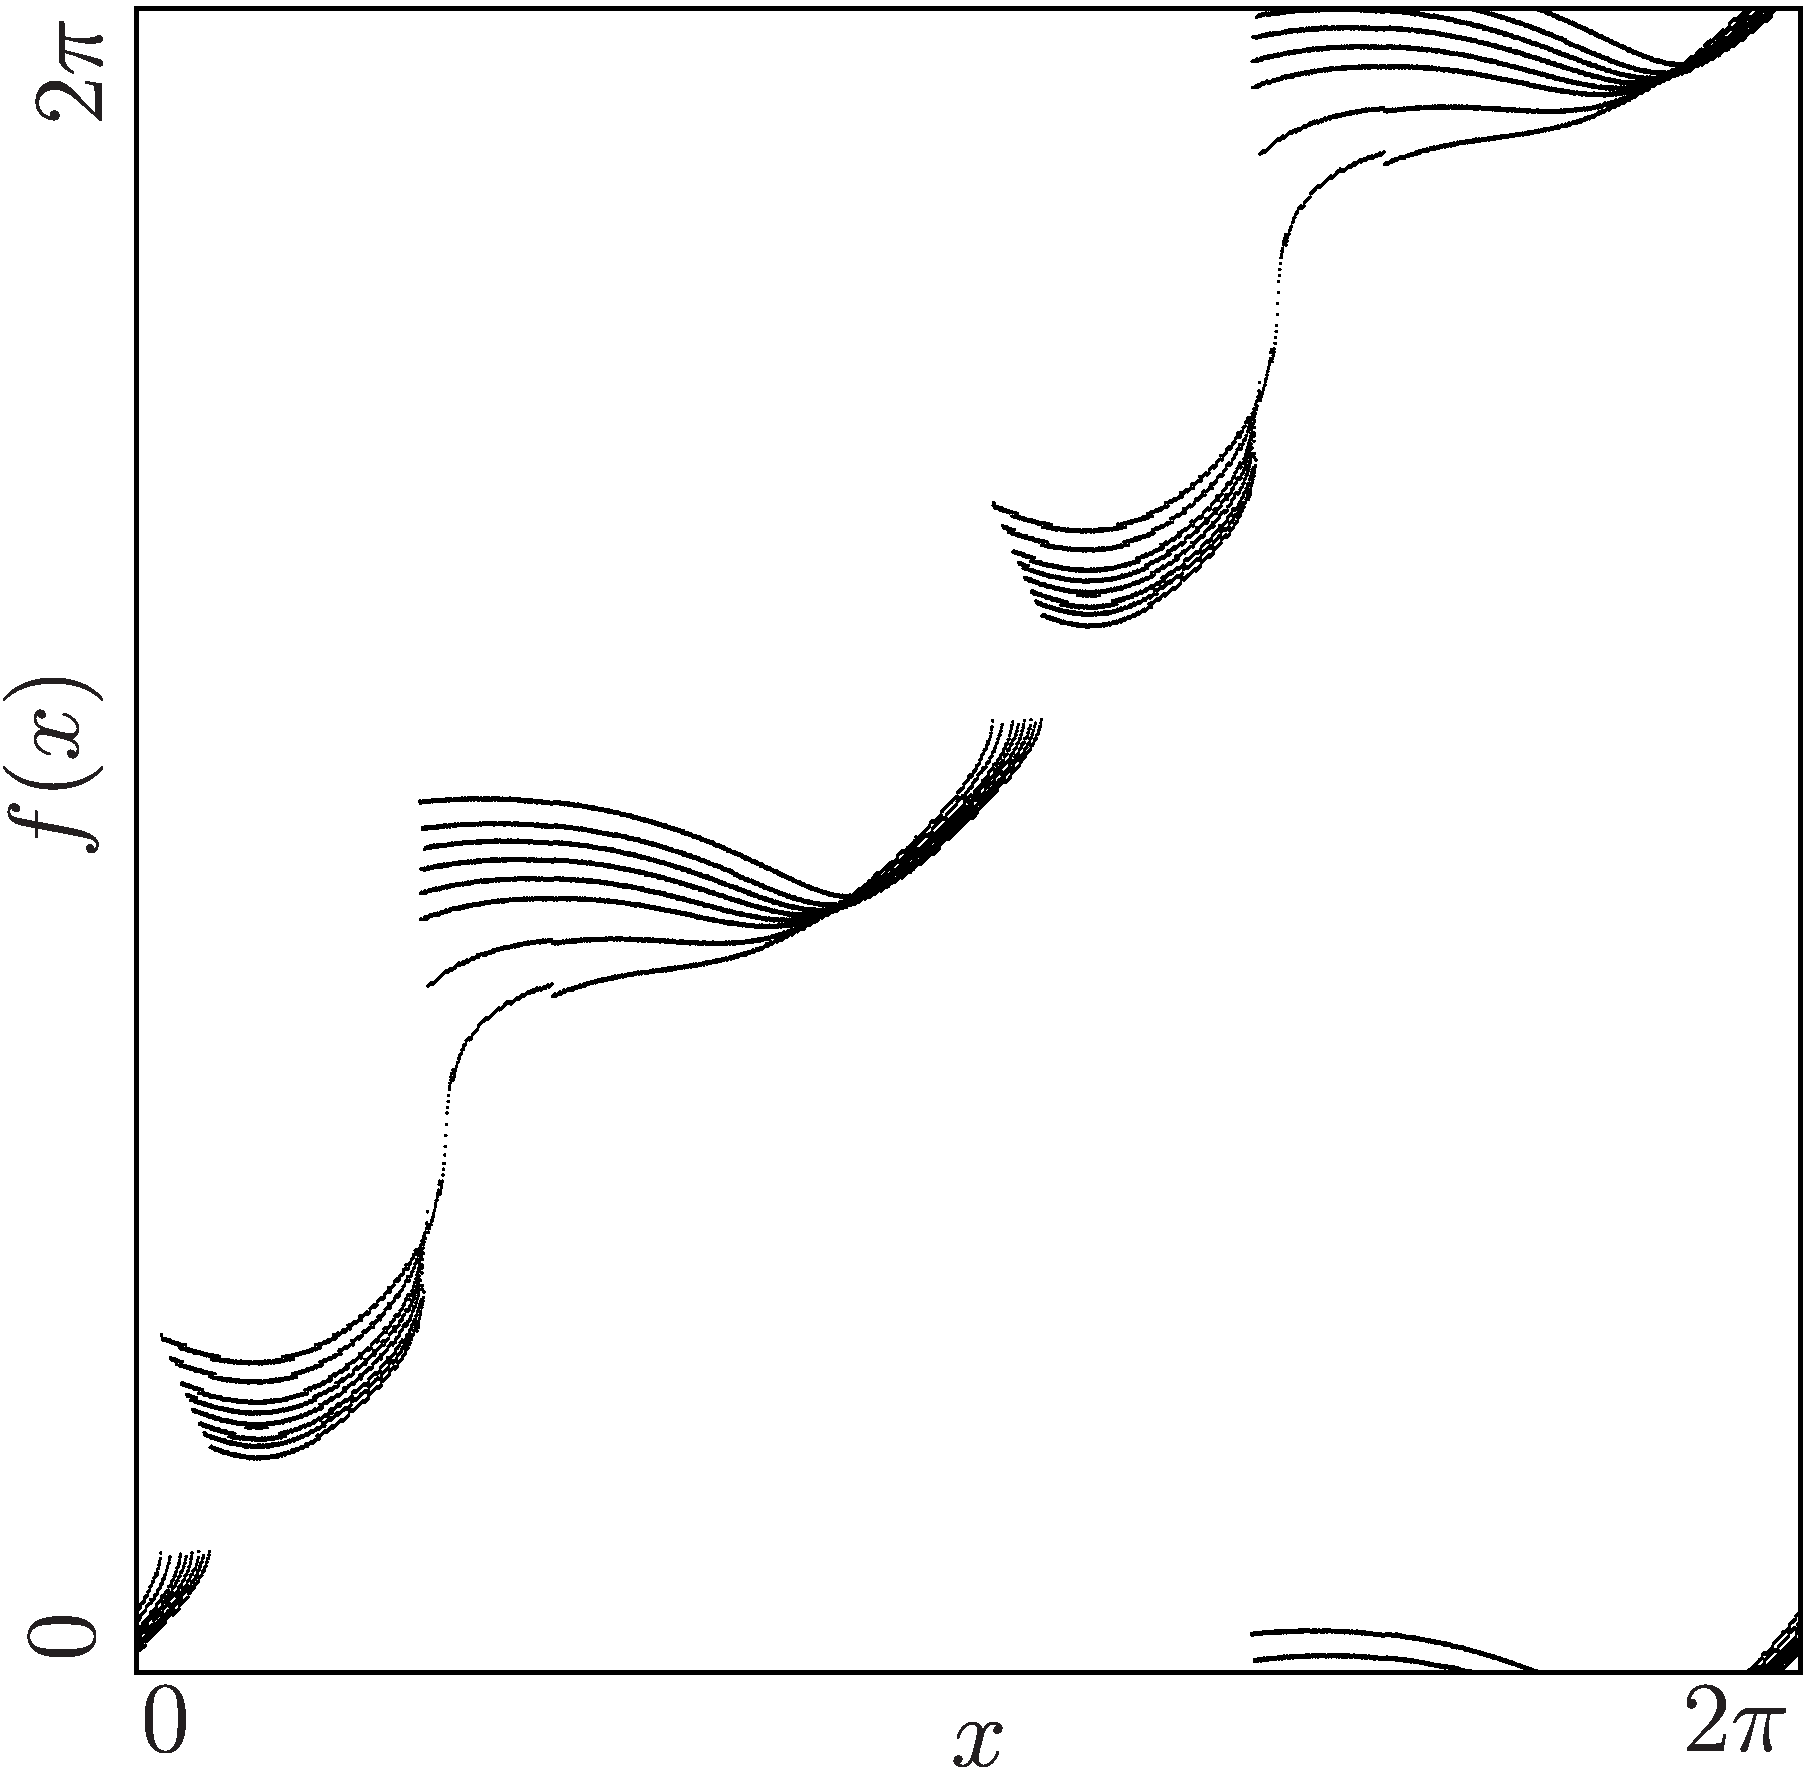
\includegraphics[height=.5 \textheight]{60_MinimalRepr/ParameterEffects/AB/illustration.png}
                \caption*{Illustration of the parameters $A$ and $B$}
            \end{figure}
        \end{column}
    \end{columns}
\end{frame}

\begin{frame}{The Next Step}
    Research question 3 remaining: What else can happen?

    \pause
    \vspace{2em}
    Hypothesis:
    \todo{motivate period adding \\ chains of same period next to each other => incrementing \\ type of map normally exhibits period adding}
    \begin{itemize}
        \item Period Adding
    \end{itemize}
\end{frame}

\begin{frame}{Symbolic Sequences}
    \todo{earlier implicit on first/second slide where type B parameter regions are mentioned?}

    Cycles are described using Symbolic Sequences.
    Sequence of Symbols indicating, on which partition of the function the points of the cycle are.
    \todo{example with graph}
\end{frame}